% Define document class and geometry
\documentclass[12pt]{article}
\usepackage[bottom = 27mm, right = 30mm, top = 27mm, left=30mm]{geometry}

% Include hyperlinks
% Source: https://ctan.org/pkg/hyperref?lang=en
\usepackage{hyperref}
\hypersetup{
	colorlinks,
	linkcolor={black},
	citecolor={black},
	urlcolor={black}
}

% To use landscape format
% Source: https://ctan.org/pkg/lscape
\usepackage{lscape}

% Animate visualizations in latex
% Source: https://ctan.org/pkg/animate
\usepackage{animate}

% Needed to produce aminations
% Source: https://ctan.org/pkg/media9
\usepackage{media9}

% Include graphs
% Source: https://ctan.org/pkg/graphicx
\usepackage{graphicx}

% Begin document
\begin{document}

% Begin landscape format
\begin{landscape}

% Page without page number
% Source: https://tex.stackexchange.com/questions/83860/remove-page-number-from-just-one-float-page
\thispagestyle{empty}

% Begin centring
\begin{center}

% Generate animations based on single frames, including a control panel
% Source: https://ctan.kako-dev.de/macros/latex/contrib/animate/animate.pdf
\animategraphics[controls={play, step, stop, speed}, loop, height=8.2cm, trim = 4cm 4.2cm 4cm 2cm, buttonsize=1em]{20}{map_capdist_}{1989}{2014}
\animategraphics[controls={play, step, stop, speed}, loop, height=8.2cm, trim = 4cm 4.2cm 4cm 2cm, buttonsize=1em]{20}{map_prec_gpcc_}{1989}{2013}
\animategraphics[controls={play, step, stop, speed}, loop, height=8.2cm, trim = 4cm 4.2cm 4cm 2cm, buttonsize=1em]{20}{map_nlights_mean_}{1992}{2013} 
\\ \vspace{0.5cm}

% Include screenshots of scatter plots, with links to animated versions of visualization
% Source: https://tex.stackexchange.com/questions/450422/include-a-html-file-in-a-latex-beamer-presentation
\hspace{0.7cm}
\href{https://www.dropbox.com/s/l9ozahng9bdyovs/capdist.html?dl=0}{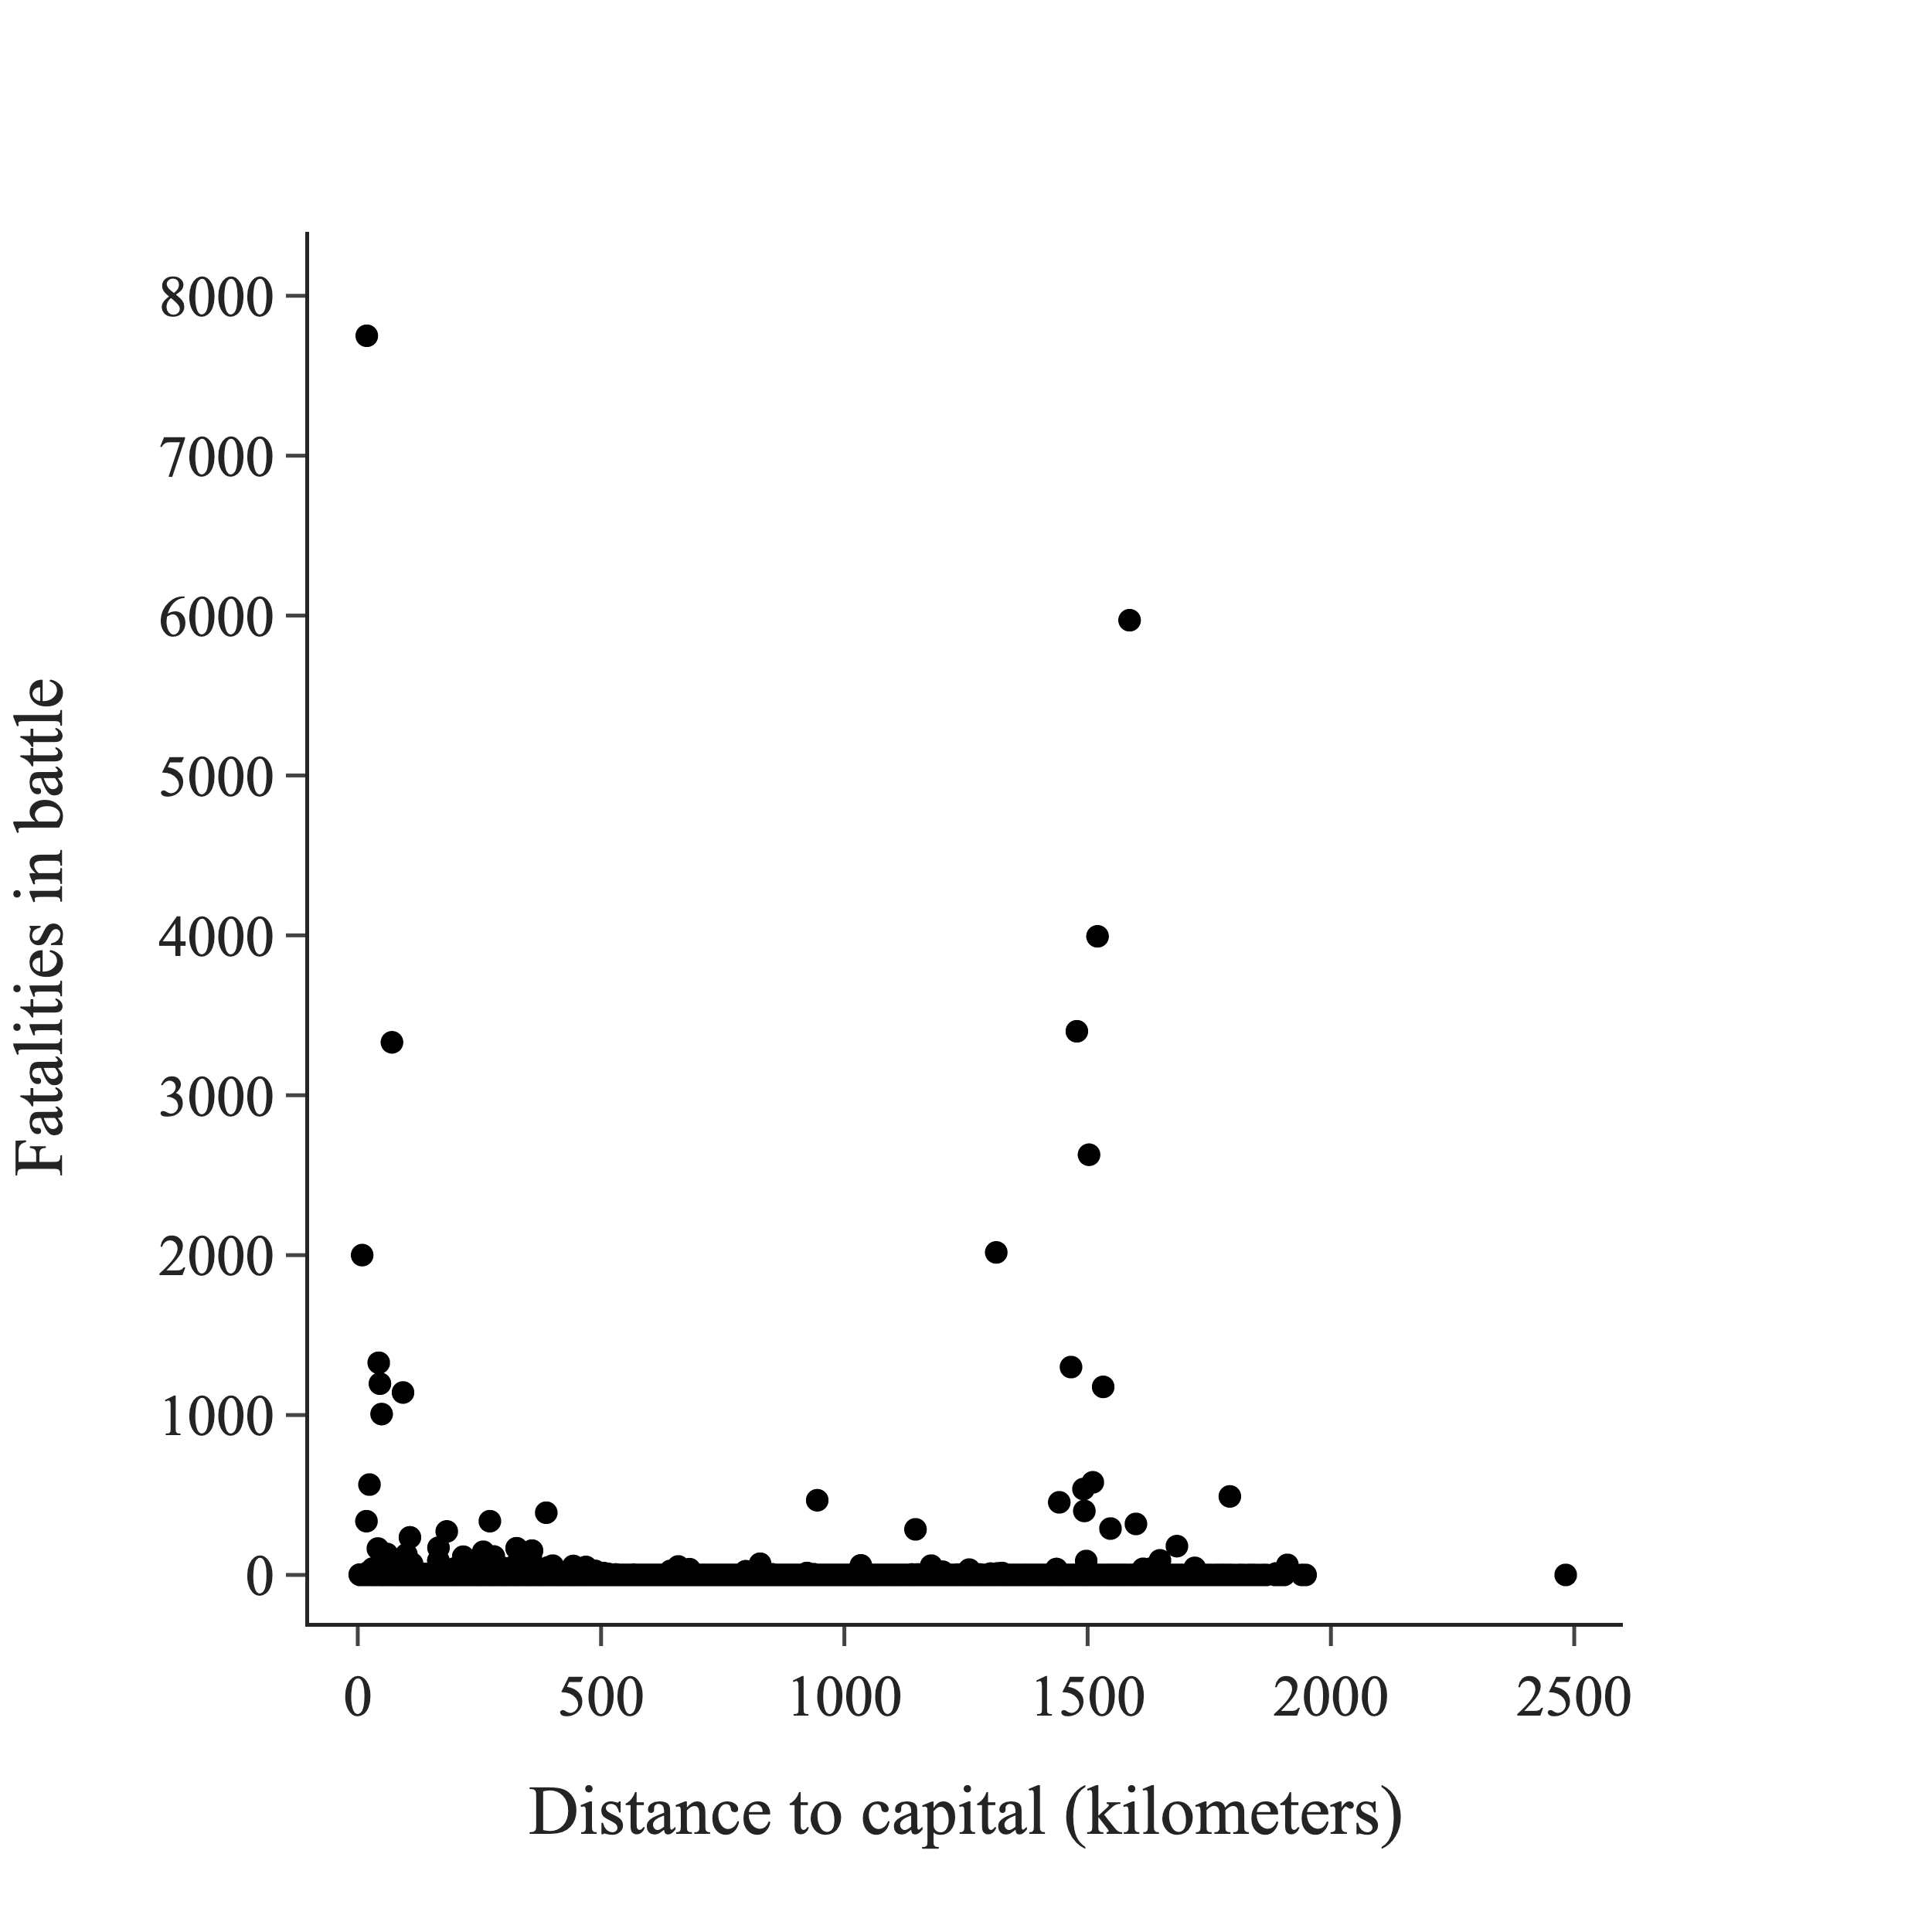
\includegraphics[scale=0.07]{capdist_1996.png}} 
\hspace{1.1cm}
\href{https://www.dropbox.com/s/7nav1uhlsocdw6u/prec_gpcc.html?dl=0}{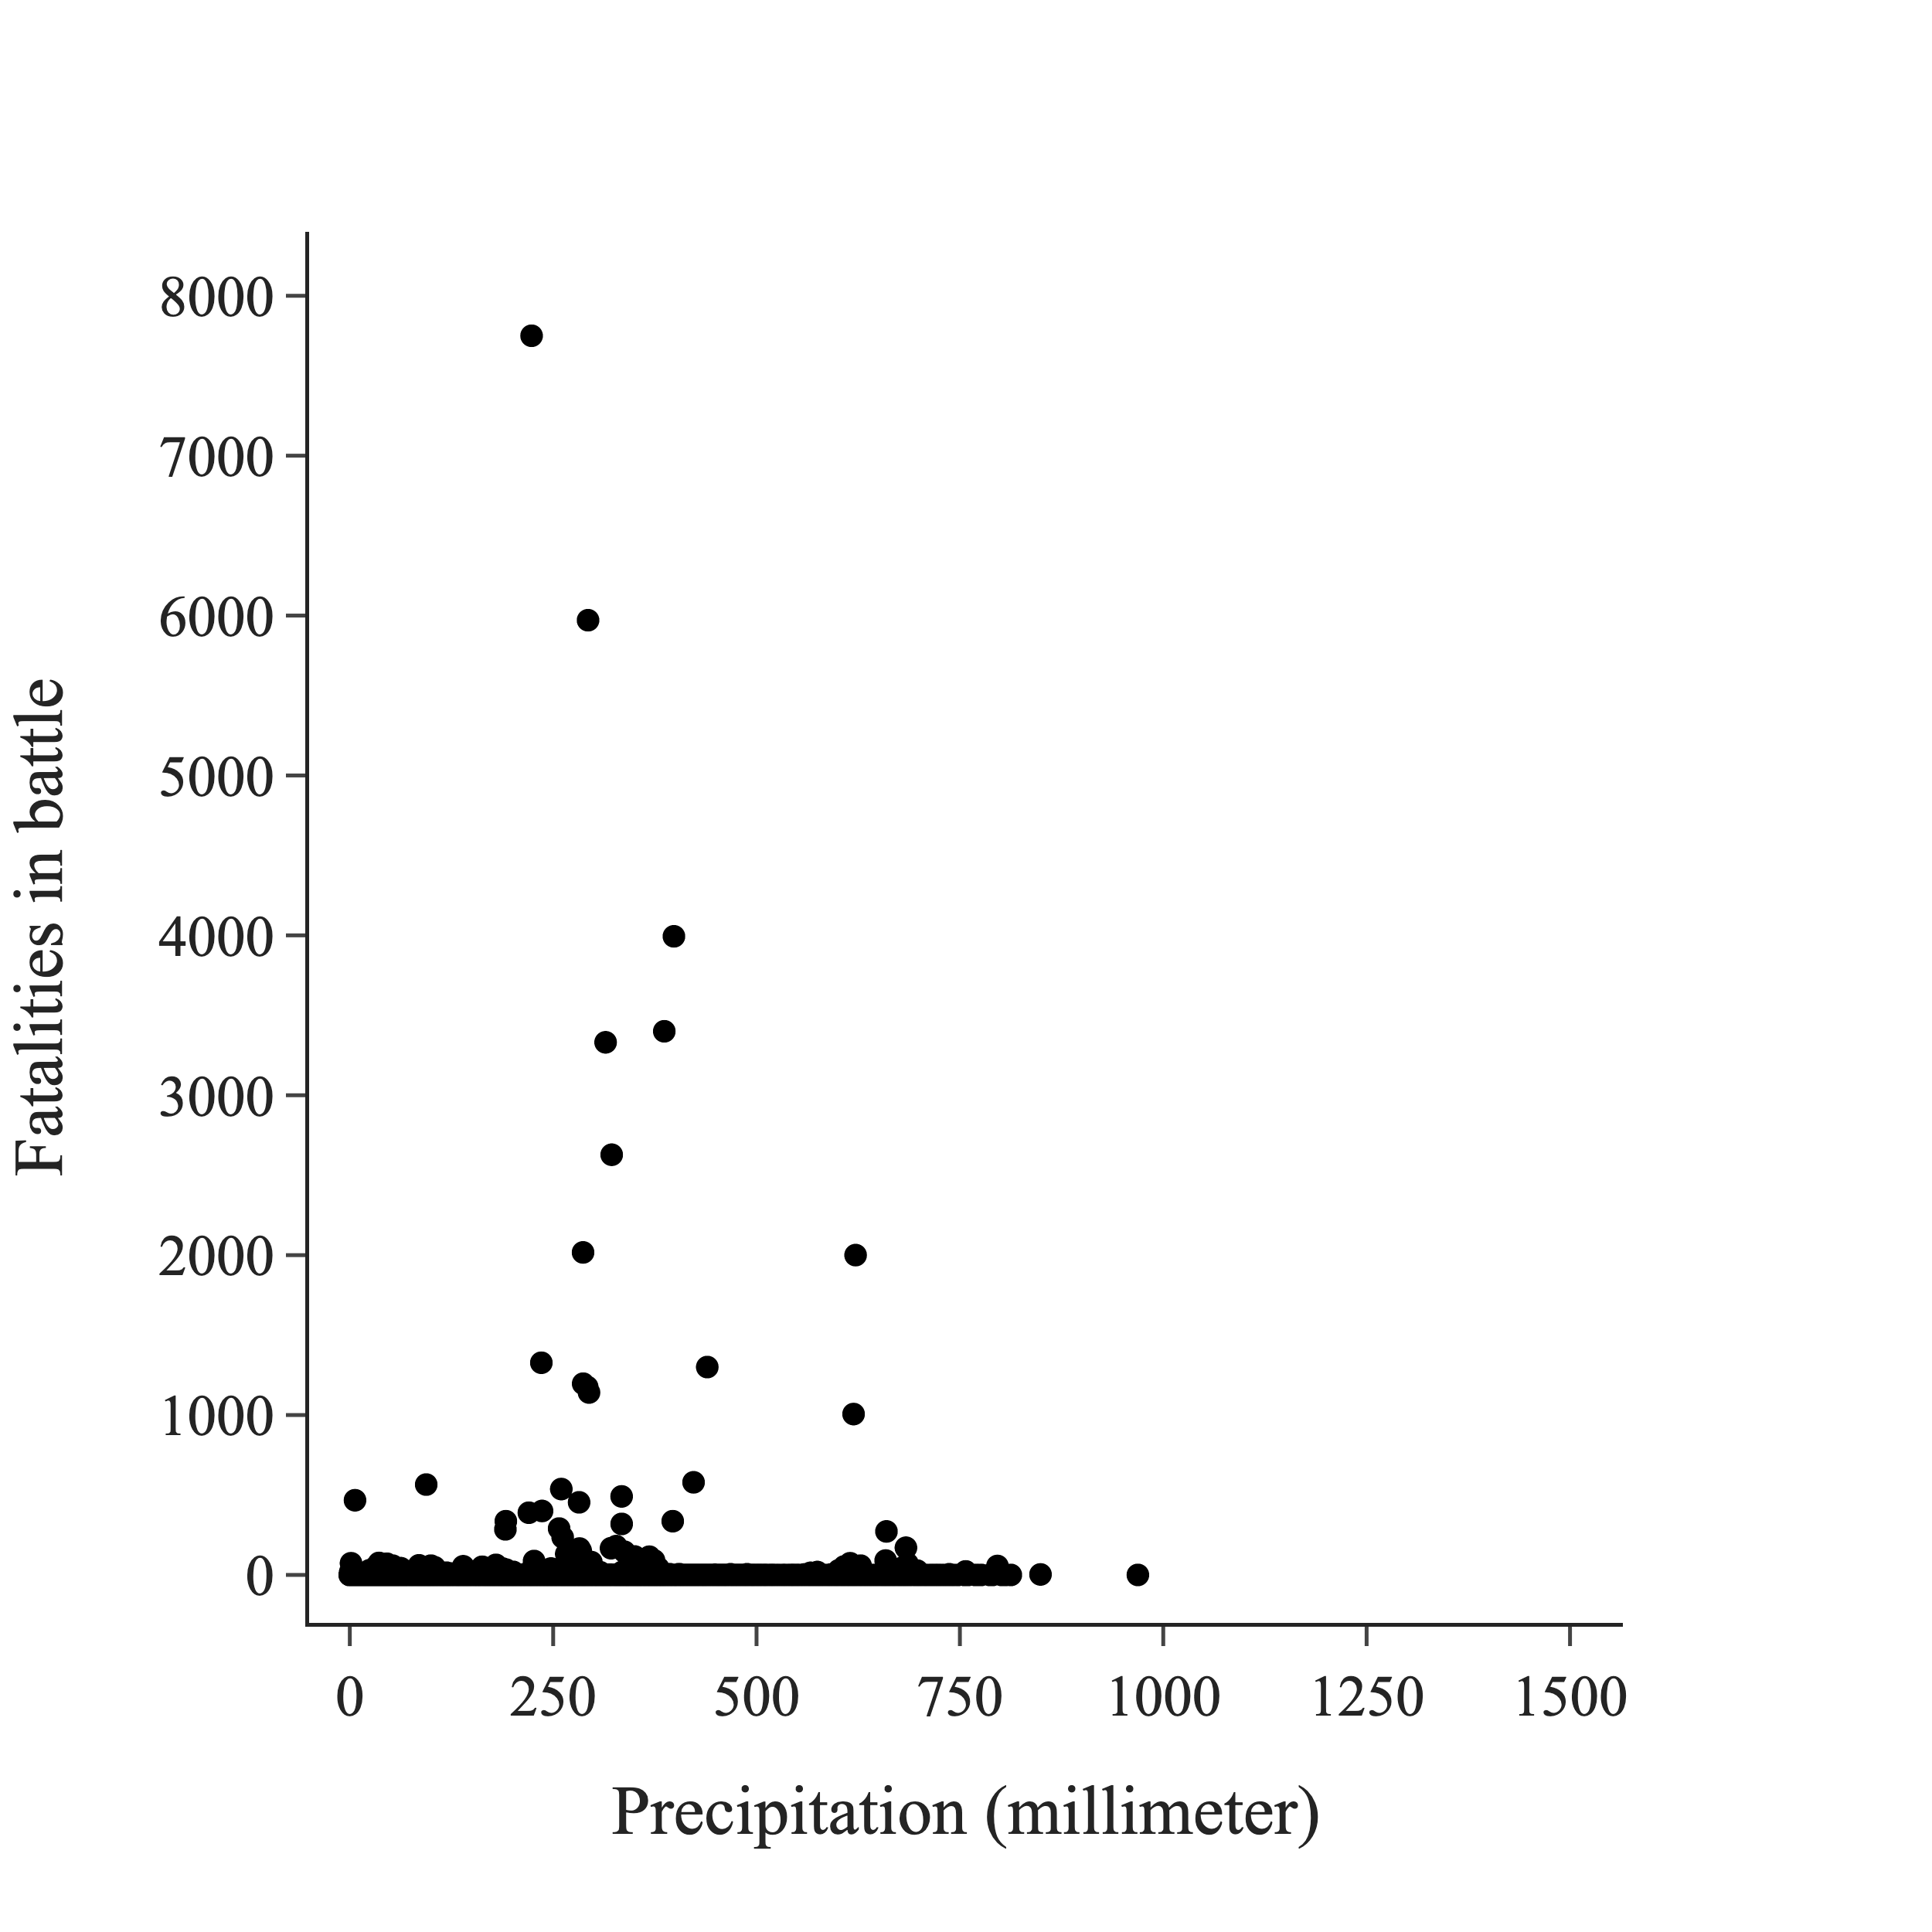
\includegraphics[scale=0.07]{prec_gpcc_1996.png}}
\hspace{1.1cm}
\href{https://www.dropbox.com/s/g7jhruocgk8mtmp/nlights_mean.html?dl=0}{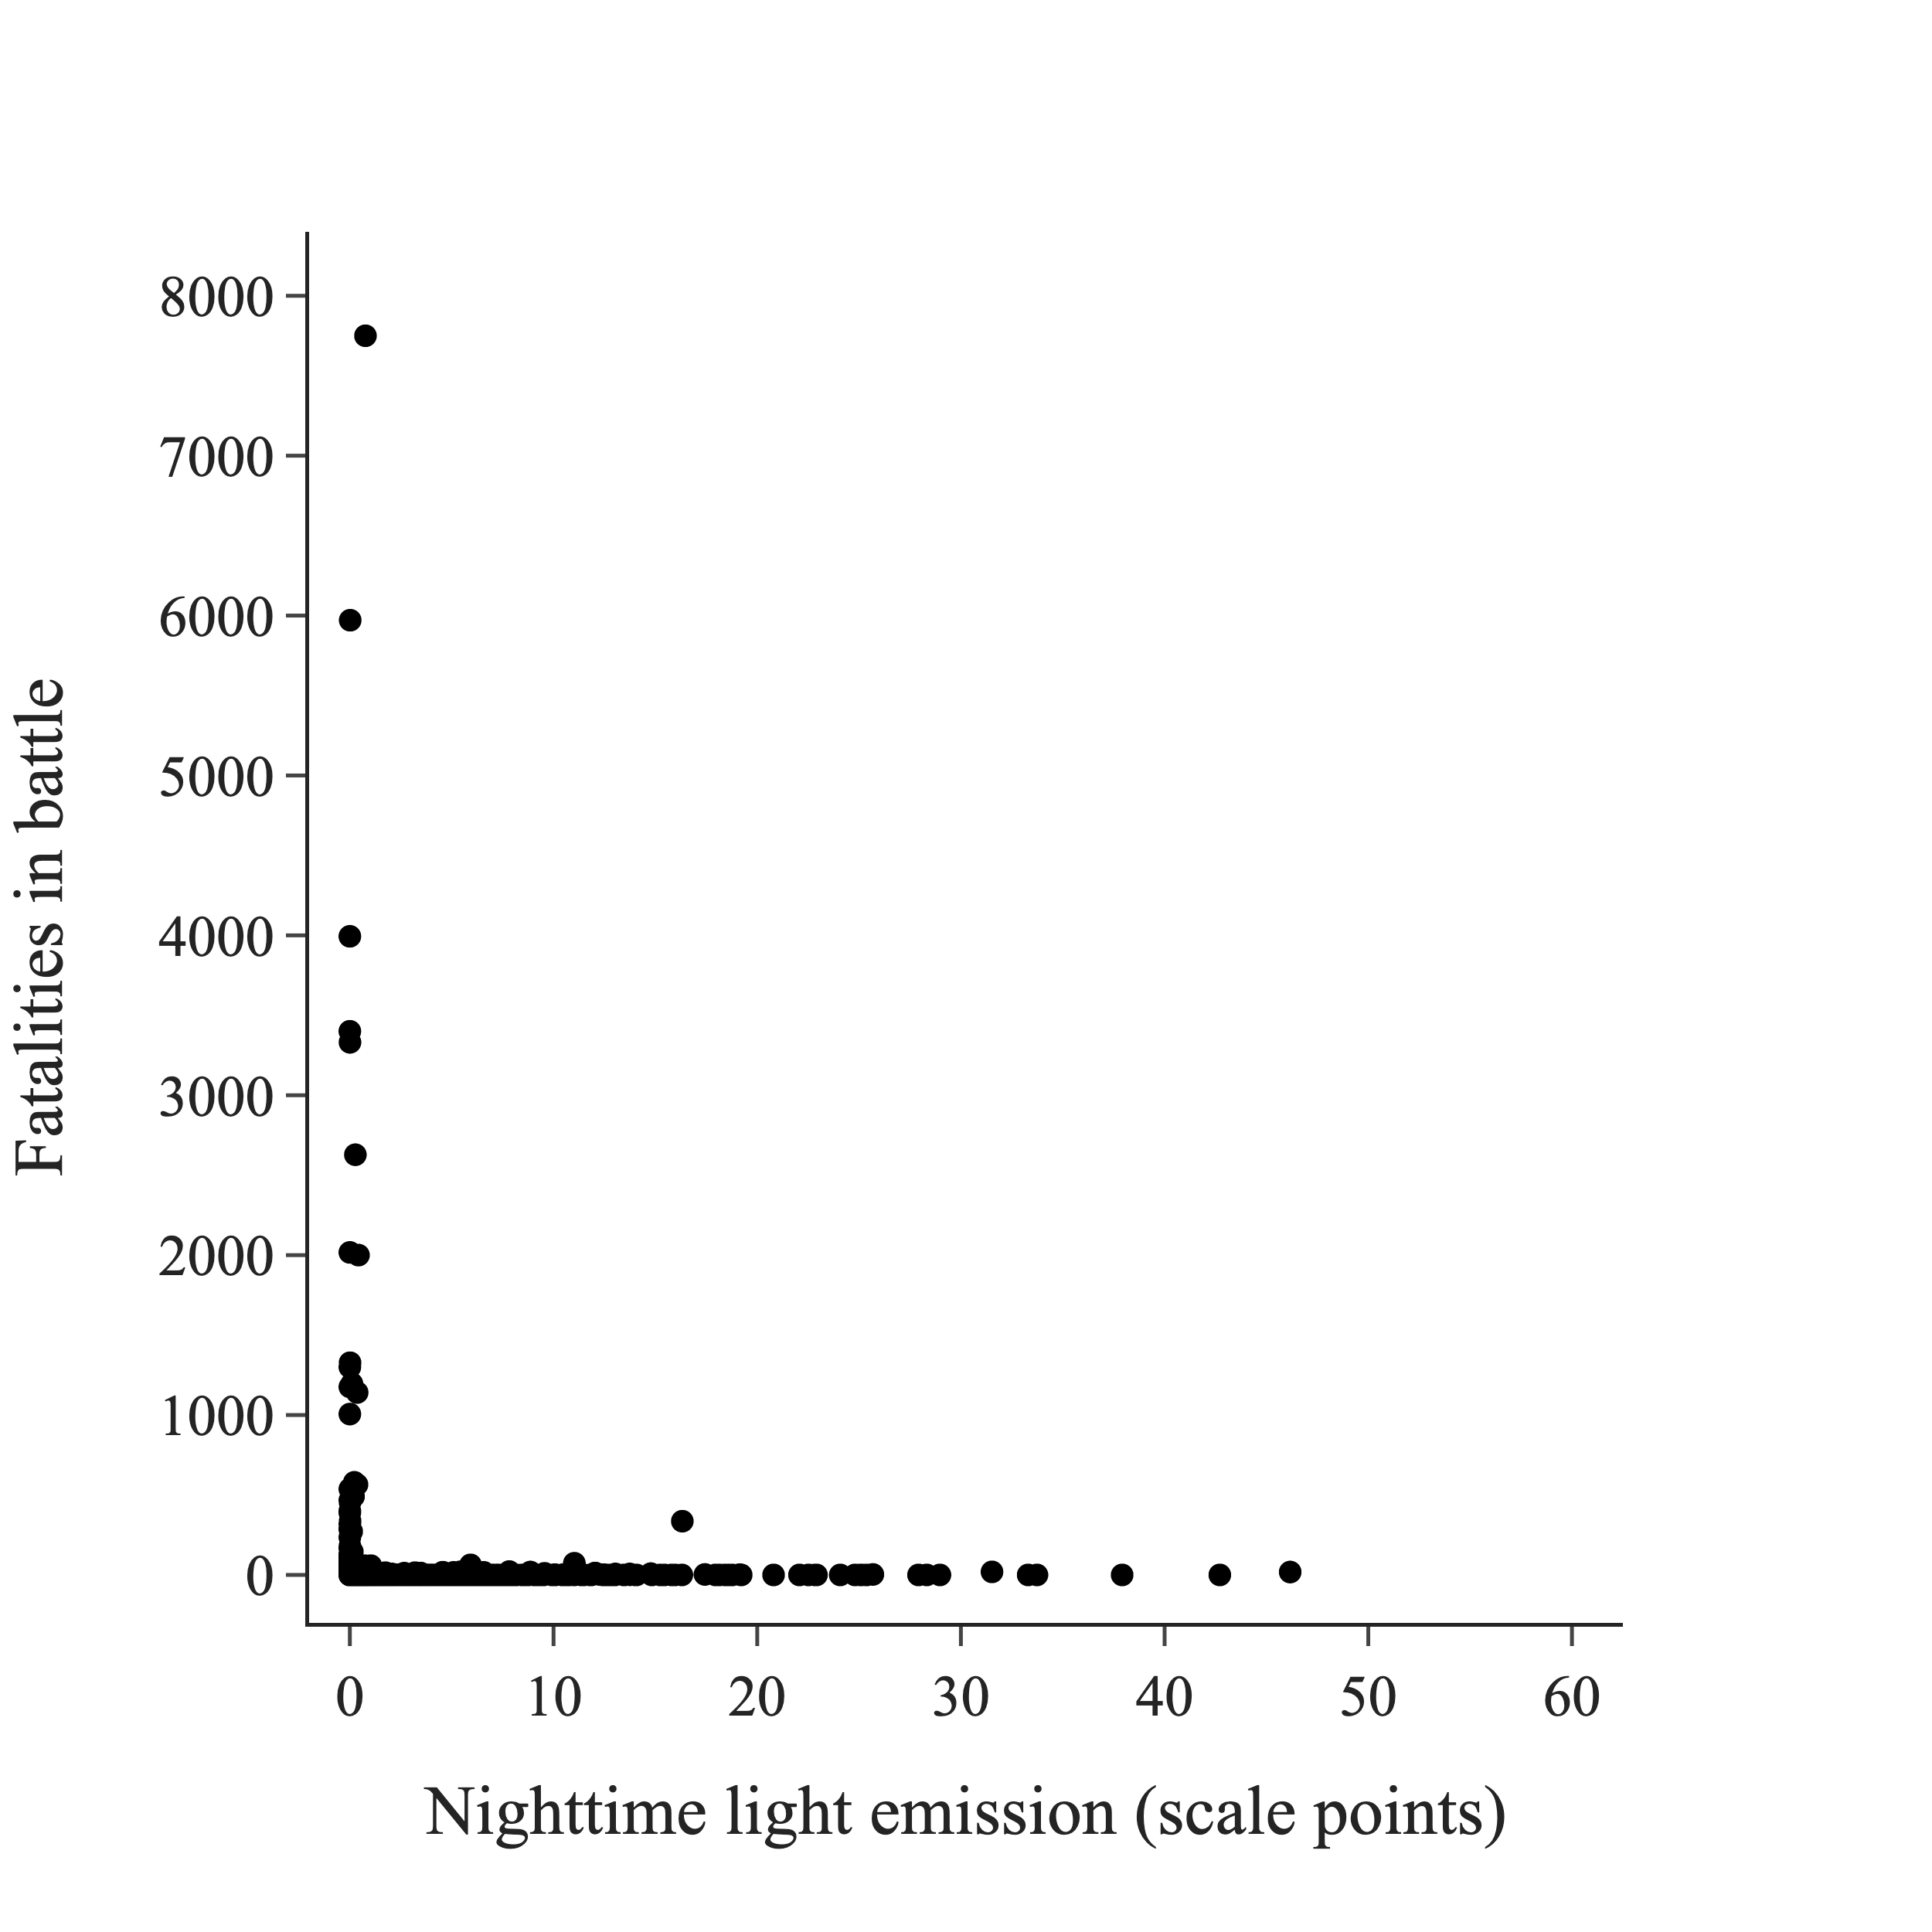
\includegraphics[scale=0.07]{nlights_mean_1996.png}}

\end{center}

\end{landscape}

\end{document}

